\documentclass[conference]{IEEEtran}
\IEEEoverridecommandlockouts
% The preceding line is only needed to identify funding in the first footnote. If that is unneeded, please comment it out.
\usepackage{cite}
\usepackage{amsmath,amssymb,amsfonts}
\usepackage{algorithmic}
\usepackage{graphicx}
\usepackage{textcomp}
\def\BibTeX{{\rm B\kern-.05em{\sc i\kern-.025em b}\kern-.08em
    T\kern-.1667em\lower.7ex\hbox{E}\kern-.125emX}}
\begin{document}

\title{CS 289A Final Project Proposal\\
Driving motion prediction using machine learning
}

\author{\IEEEauthorblockN{Jessica Leu}
\IEEEauthorblockA{\textit{SID : 3033088125} \\
jess.leu24@berkeley.edu}
\and
\IEEEauthorblockN{2\textsuperscript{nd} Given Name Surname}
\IEEEauthorblockA{\textit{SID : 3033088125} \\
jess.leu24@berkeley.edu}
\and
\IEEEauthorblockN{3\textsuperscript{rd} Given Name Surname}
\IEEEauthorblockA{\textit{SID : 3033088125} \\
jess.leu24@berkeley.edu}
\and
\IEEEauthorblockN{4\textsuperscript{th} Given Name Surname}
\IEEEauthorblockA{\textit{SID : 3033088125} \\
jess.leu24@berkeley.edu}
}

\maketitle

\begin{abstract}
This work proposed a method to predict a car's trajectory based on observation of its previous trajectory and the surrounding car's motion. The car's behavior, or driving policy, is modeled as an motion planning optimization problem. The parameters in the optimization problem indicate the driver's characteristic. In this work, parameter ranges for different types of driver are defined. Training trajectories and driver type labels are generated by simulation. Later on, a neural net is trained to learn the policy for predicting the driver's type based on observed trajectory. Finally, motion prediction can be made with the predicted driver type.
\end{abstract}

\begin{IEEEkeywords}
Machine learning, motion prediction, motion planing
\end{IEEEkeywords}

\section{Idea}
As the research field of autonomous driving gets more and more vibrant, motion prediction of the surrounding vehicle also arises as one of the hardest problem that need to be solved. Many attempts have been made, people tried to classify drivers' type as being constrictive, neutral, or aggressive base on their driving motion. Knowing the fact that many control engineers actually do motion planing by solving an optimization problem, we come up with an idea that we can model all the cars' motion, both human driving car and autonomous driving car, as the optimal trajectory generated by solving an optimization problem (i.e. driving policy of the car). And the parameters in the cost function and constraints are what characterize the driver's tpye. Therefore, the proposed method is done through the following steps. First, define parameter range for several different types of driver. Second, learn the relation between the parameters in the optimization problem and the output optimal trajectory from the generated training data. Third, predict the parameters in the driving policy of a new car based on some observation of its previous motion. Forth, classify the driver's type based on the predicted parameters. Finally, predict the future trajectory of the new car based on its type. 

\section{Problem Description}
Among all the setting in autonomous driving scenes, one of the most complicated one is at an intersection with only stop signs and no traffic light. A scenario is shown in Fig.1, where the car on the left (target car) suddenly encounters a car coming from its left in a high speed and doesn't seem to stop. In the simplest case, the target car will have two choices, one is to stop immediately and let the crazy car go first, another choice is to continue moving forward but deviates a bit to avoid collision. The decision made by the target car will influence the decision making of the ego car. If the target car decides to stop, the ego car can go straight, while in the other case the ego car should better stop. Therefore, the ego car's prediction of the target car becomes important.
\begin{figure}[h!]
\centering
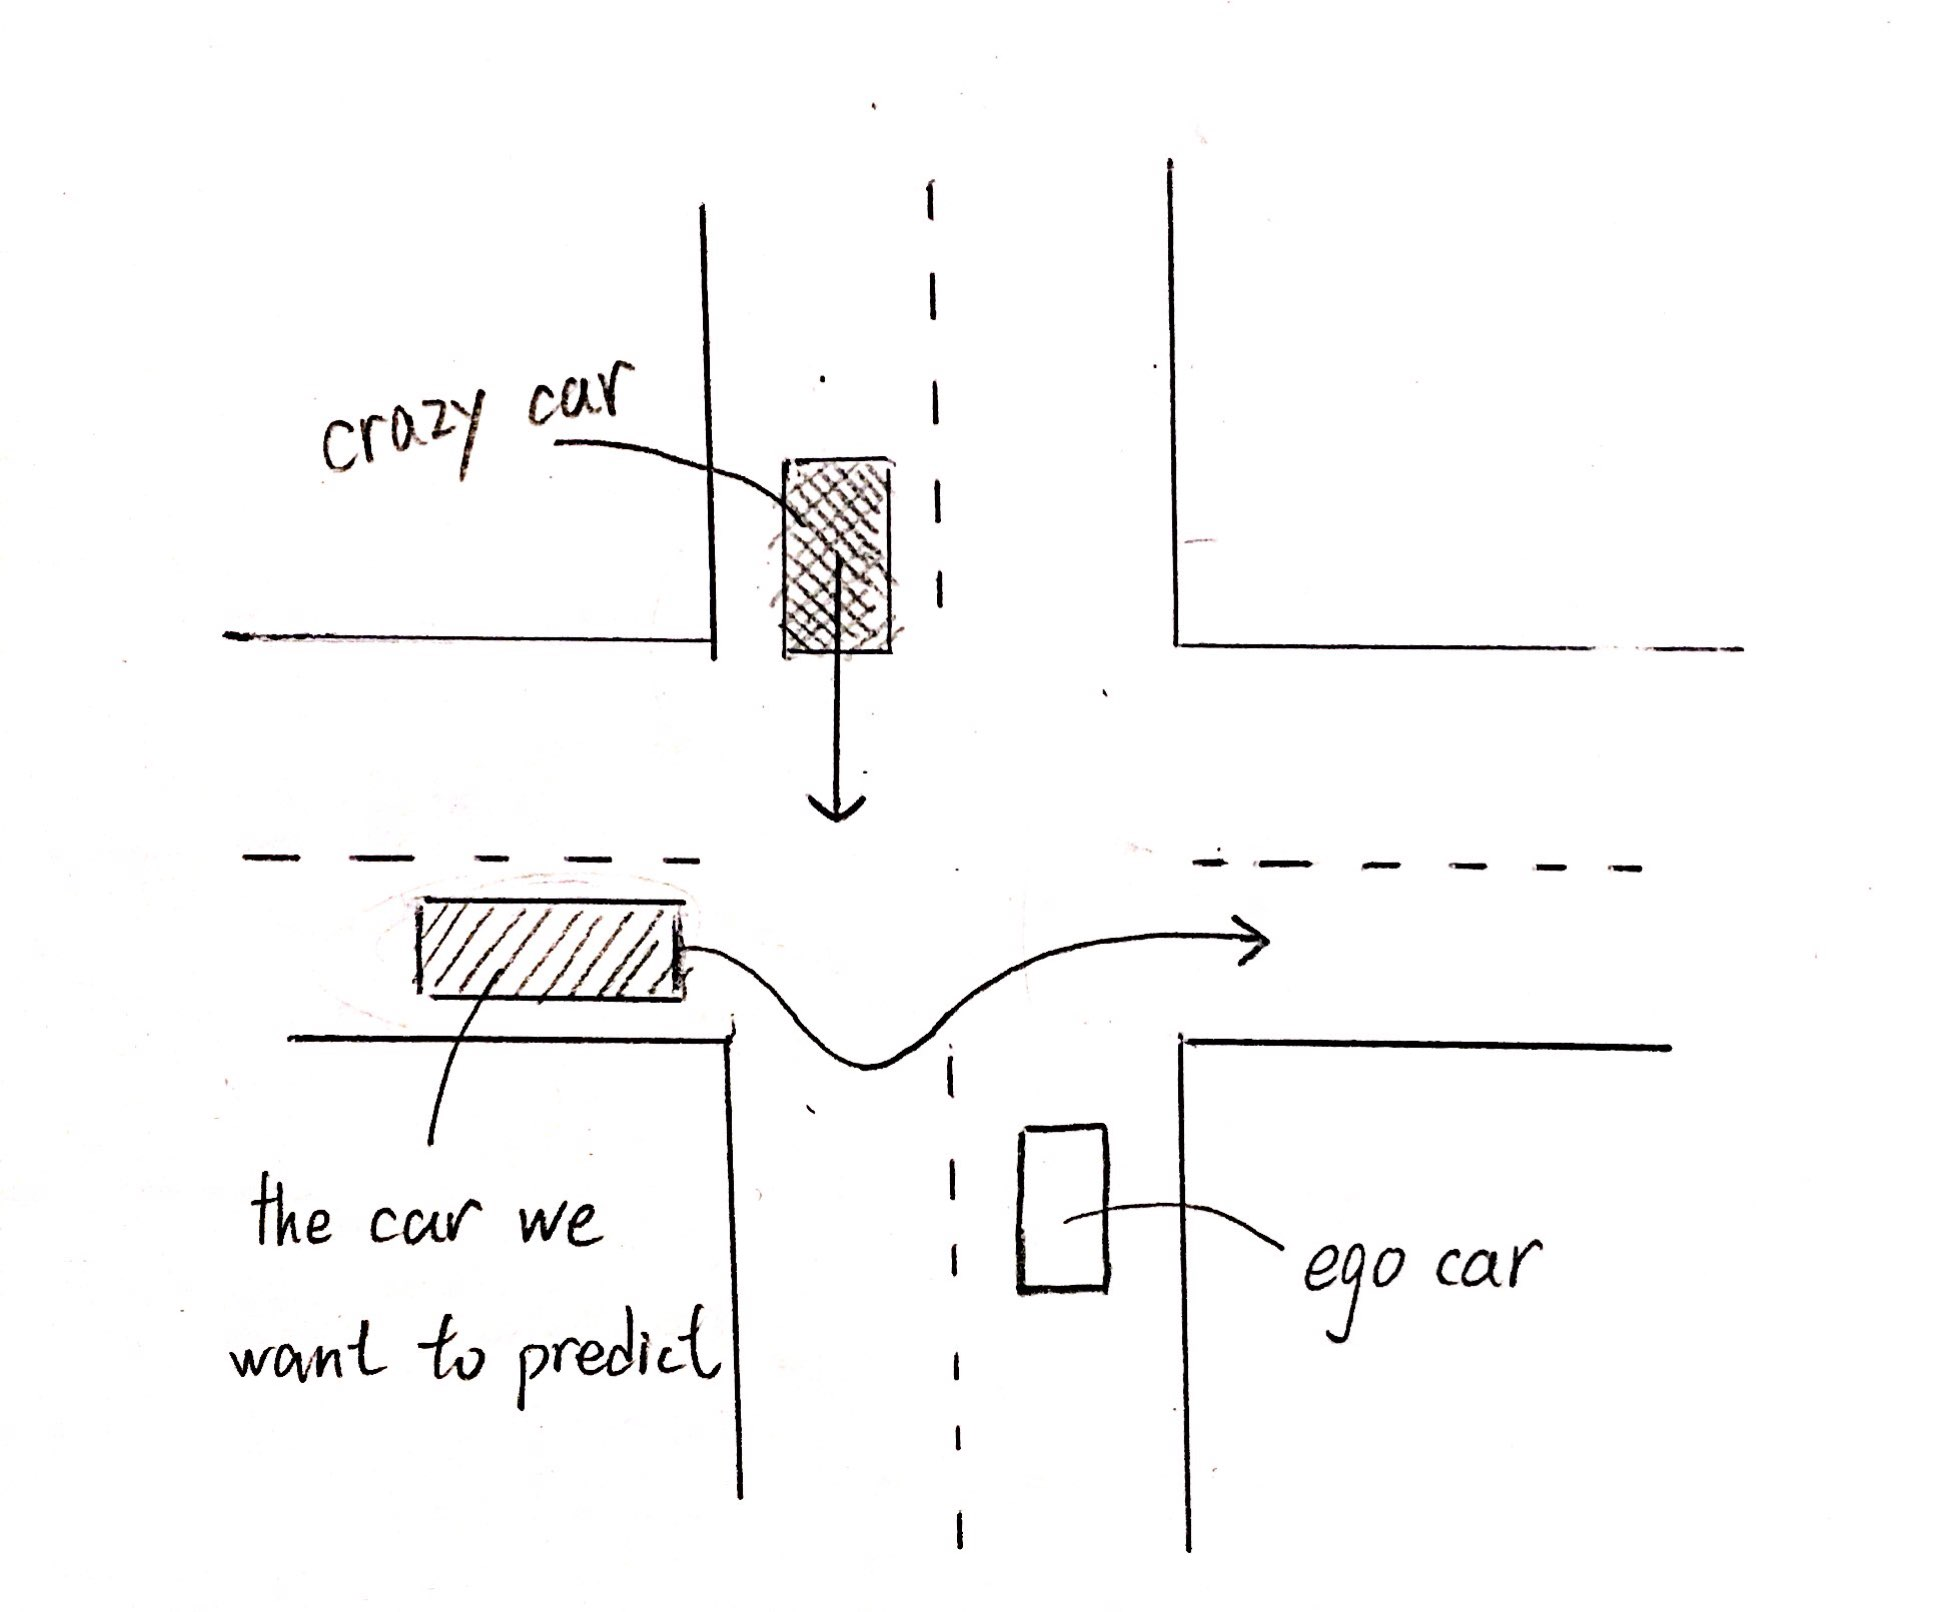
\includegraphics[scale = 0.1]{problem.png}
\caption{We use the BARC vehicle as an experimental platform for MPC for lateral reference tracking.}
\label{fig:reftraj}
\end{figure}

\section{Methods}

\subsection{Type defining and data generation}

According to general driving rules in the U.S., we can roughly classify drivers into three types, constrictive, neutral, and aggressive. The training data is generated by doing simulation of motion planning. The motion planning is done by a control frame work called Model Predictive Control (MPC), which is largely used in industry. The idea of this MPC frame work is to solve an optimization problem that outputs the optimal trajectory for some number of future step. Assuming that the car has preformed tracking for the first step, the optimization problem will take the current position as a feedback and solve the optimization problem again. In this work, we set the parameters and construct the optimization problem according to the label, the driver's type, and run the simulation to generate the corresponding output trajectory. After this process, we have our training trajectories and labels.

\section{Methods}

\subsection{Type defining and data generation}

According to general driving rules in the U.S., we can roughly classify drivers into three types, constrictive, neutral, and aggressive. The training data is generated by doing simulation of motion planning. The motion planning is done by a control frame work called Model Predictive Control (MPC), which is largely used in industry. The idea of this MPC frame work is to solve an optimization problem that outputs the optimal trajectory for some number of future step. Assuming that the car has preformed tracking for the first step, the optimization problem will take the current position as a feedback and solve the optimization problem again. In this work, we set the parameters and construct the optimization problem according to the label, the driver's type, and run the simulation to generate the corresponding output trajectory. After this process, we have our training trajectories and labels.

\section{Prepare Your Paper Before Styling}
Before you begin to format your paper, first write and save the content as a 
separate text file. Complete all content and organizational editing before 
formatting. Please note sections \ref{AA}--\ref{SCM} below for more information on 
proofreading, spelling and grammar.

Keep your text and graphic files separate until after the text has been 
formatted and styled. Do not number text heads---{\LaTeX} will do that 
for you.

\subsection{Abbreviations and Acronyms}\label{AA}
Define abbreviations and acronyms the first time they are used in the text, 
even after they have been defined in the abstract. Abbreviations such as 
IEEE, SI, MKS, CGS, ac, dc, and rms do not have to be defined. Do not use 
abbreviations in the title or heads unless they are unavoidable.

\subsection{Units}
\begin{itemize}
\item Use either SI (MKS) or CGS as primary units. (SI units are encouraged.) English units may be used as secondary units (in parentheses). An exception would be the use of English units as identifiers in trade, such as ``3.5-inch disk drive''.
\item Avoid combining SI and CGS units, such as current in amperes and magnetic field in oersteds. This often leads to confusion because equations do not balance dimensionally. If you must use mixed units, clearly state the units for each quantity that you use in an equation.
\item Do not mix complete spellings and abbreviations of units: ``Wb/m\textsuperscript{2}'' or ``webers per square meter'', not ``webers/m\textsuperscript{2}''. Spell out units when they appear in text: ``. . . a few henries'', not ``. . . a few H''.
\item Use a zero before decimal points: ``0.25'', not ``.25''. Use ``cm\textsuperscript{3}'', not ``cc''.)
\end{itemize}



\section*{References}

Please number citations consecutively within brackets \cite{b1}. The 
sentence punctuation follows the bracket \cite{b2}. Refer simply to the reference 
number, as in \cite{b3}---do not use ``Ref. \cite{b3}'' or ``reference \cite{b3}'' except at 
the beginning of a sentence: ``Reference \cite{b3} was the first $\ldots$''

Number footnotes separately in superscripts. Place the actual footnote at 
the bottom of the column in which it was cited. Do not put footnotes in the 
abstract or reference list. Use letters for table footnotes.

Unless there are six authors or more give all authors' names; do not use 
``et al.''. Papers that have not been published, even if they have been 
submitted for publication, should be cited as ``unpublished'' \cite{b4}. Papers 
that have been accepted for publication should be cited as ``in press'' \cite{b5}. 
Capitalize only the first word in a paper title, except for proper nouns and 
element symbols.

For papers published in translation journals, please give the English 
citation first, followed by the original foreign-language citation \cite{b6}.

\begin{thebibliography}{00}
\bibitem{b1} G. Eason, B. Noble, and I. N. Sneddon, ``On certain integrals of Lipschitz-Hankel type involving products of Bessel functions,'' Phil. Trans. Roy. Soc. London, vol. A247, pp. 529--551, April 1955.
\bibitem{b2} J. Clerk Maxwell, A Treatise on Electricity and Magnetism, 3rd ed., vol. 2. Oxford: Clarendon, 1892, pp.68--73.
\bibitem{b3} I. S. Jacobs and C. P. Bean, ``Fine particles, thin films and exchange anisotropy,'' in Magnetism, vol. III, G. T. Rado and H. Suhl, Eds. New York: Academic, 1963, pp. 271--350.
\bibitem{b4} K. Elissa, ``Title of paper if known,'' unpublished.
\bibitem{b5} R. Nicole, ``Title of paper with only first word capitalized,'' J. Name Stand. Abbrev., in press.
\bibitem{b6} Y. Yorozu, M. Hirano, K. Oka, and Y. Tagawa, ``Electron spectroscopy studies on magneto-optical media and plastic substrate interface,'' IEEE Transl. J. Magn. Japan, vol. 2, pp. 740--741, August 1987 [Digests 9th Annual Conf. Magnetics Japan, p. 301, 1982].
\bibitem{b7} M. Young, The Technical Writer's Handbook. Mill Valley, CA: University Science, 1989.
\end{thebibliography}

\end{document}
